\documentclass{beamer}

\usepackage{graphicx}
\usepackage{tikz}

\usetheme{Frankfurt}

\title{The Scrum Method}
\author{Jimmy Mousel, Colin Holler, Dimitri Klockenbring, Jérémie Muzet, Céline Van Landeghem}
\date{}



\begin{document}

\frame{\titlepage}



\section{Summary}

\begin{frame}
    \frametitle{Table of content}
    \tableofcontents
\end{frame}



\section{What is Scrum?}

\begin{frame}
    \frametitle{What is Scrum ?}
    \begin{block}
        \onslide<1-> Scrum is one of the most used agile method.
        \begin{center}
            \onslide<1-> Empiricism \onslide<1-> - Participation \onslide<1-> - Self-organization
        \end{center}
    \end{block}
    \pause
    \begin{block}
        \onslide<2-> Scrum can be broken down into
        \begin{center}
            \onslide<2-> Roles \onslide<2-> - Events \onslide<2-> - Artifacts
        \end{center}
    \end{block}
\end{frame}

\begin{frame}
	\frametitle{What is Scrum ?}
	
	\framesubtitle{Roles}
	\begin{columns}
	    \column{.5\textwidth}
	    \begin{block}{Roles}
		\begin{itemize}
		    \item Product Owner
		    
		    \item Scrum Master
		    
		    \item Development Team
		\end{itemize}
	    \end{block}
	
	
	    \column{.5\textwidth}
	    
    
	    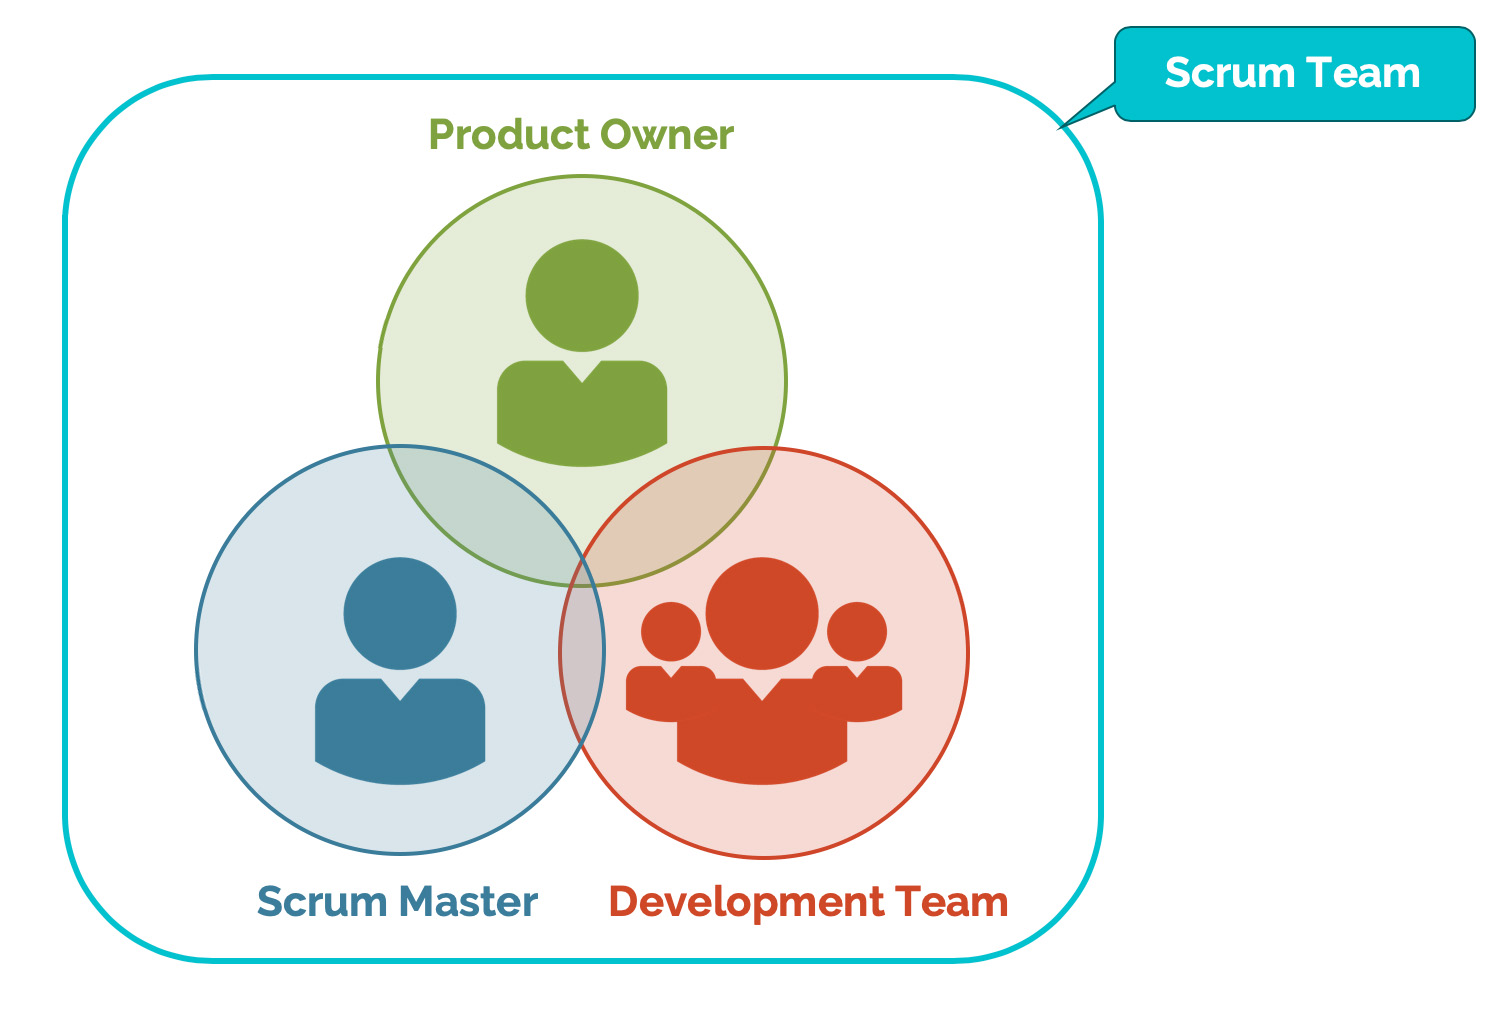
\includegraphics[width=1\textwidth]{Images/roles.jpg}   
    
	\end{columns}	
\end{frame}
    
    
    
\section{The Scrum Workflow}

\begin{frame}
\frametitle{Second slide}
\begin{center}
	% à ordonner correctement :%
	% l'origine est en bas à gauche %
	% juste à gauche de "rectangle" on met les coordonnées du coin inf gauche
	% juste à droite de "rectangle" on met les coordonnées du point sup droit
	% Dans les chevrons après "draw" on indique à quel moment ça s'affiche

	\begin{tikzpicture}
	\node[anchor=south west,inner sep=0] at (0,0) {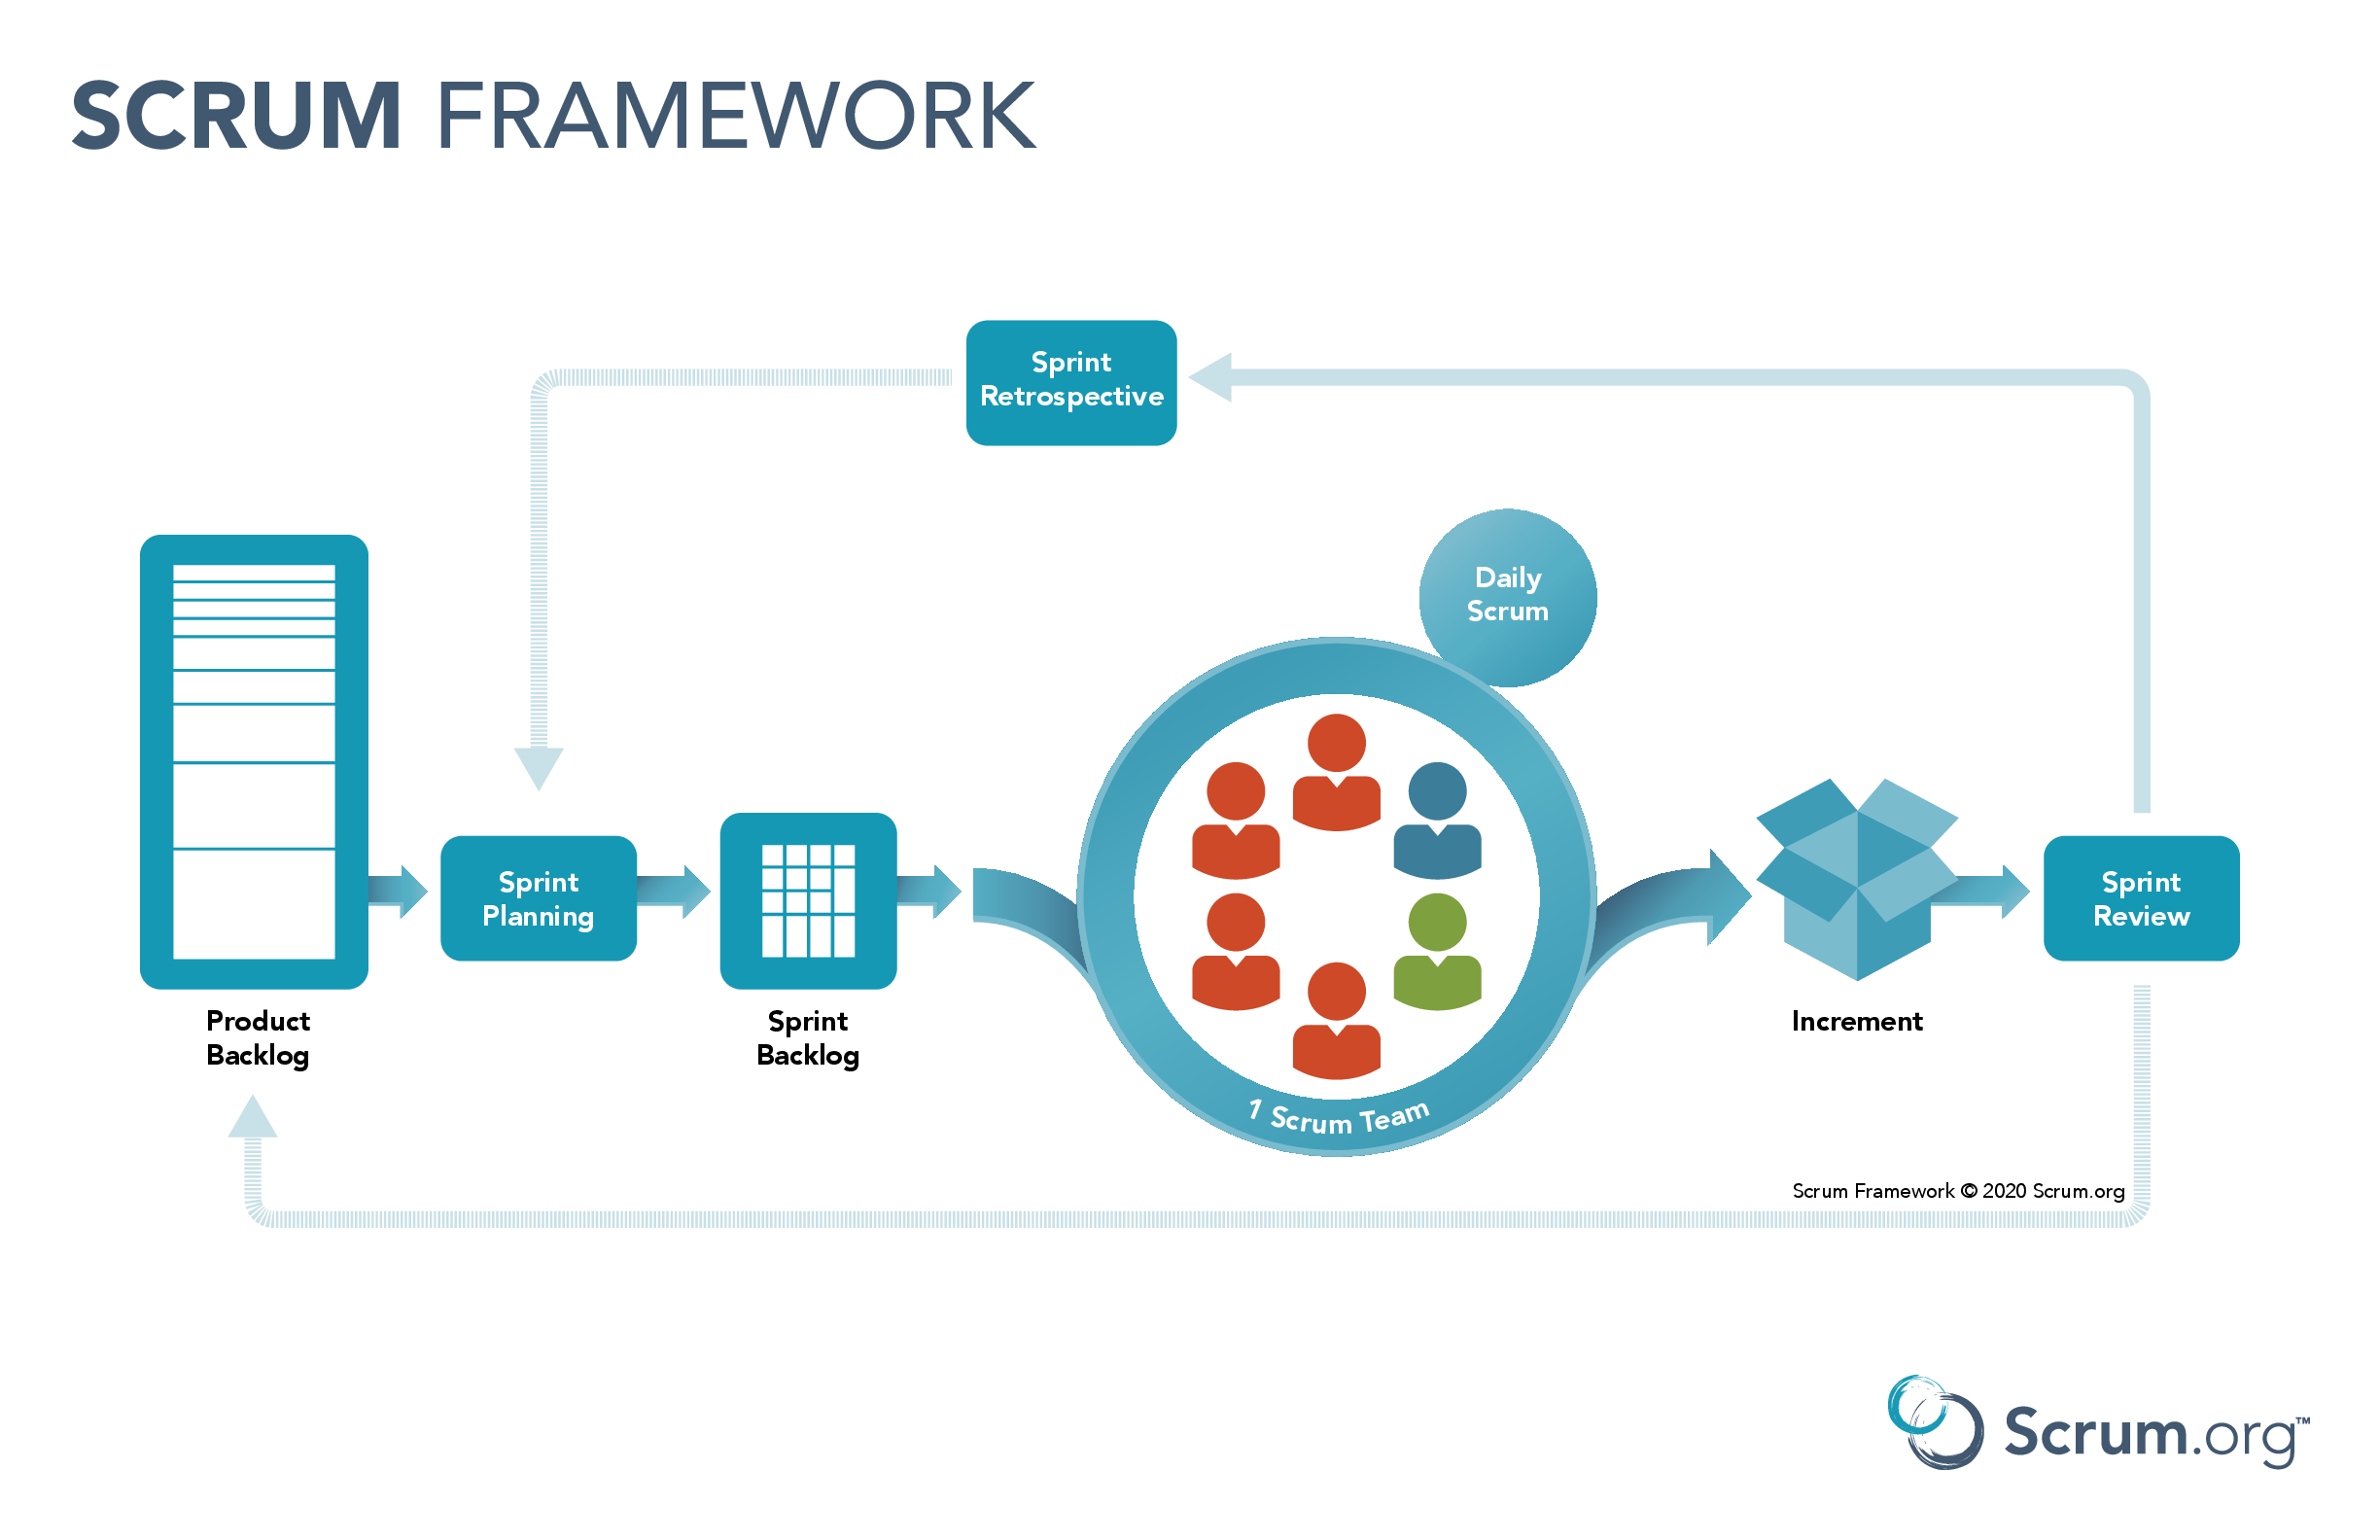
\includegraphics[width=1\textheight]{Images/Scrumorg-Scrum-Framework}};
	\draw<1>[red,ultra thick,rounded corners] (0.4,1.6) rectangle (1.5,4);
	\draw<2>[red,ultra thick,rounded corners] (1.5,2) rectangle (2.5, 2.8);

	\draw<3>[red,ultra thick,rounded corners] (2.6,1.6) rectangle (3.5, 2.9);
	\draw<4>[red,ultra thick,rounded corners] (5.2,3.1) rectangle (6.1, 4);
	\draw<5>[red,ultra thick,rounded corners] (6.5,1.7) rectangle (7.5, 3);
	\draw<6>[red,ultra thick,rounded corners] (7.5,2) rectangle (8.5, 2.8);
	\draw<7>[red,ultra thick,rounded corners] (3.5,4) rectangle (4.5, 4.7);

	\draw<8>[red,ultra thick,rounded corners] (1.5,2) rectangle (2.5, 2.8);
	\draw<9>[red,ultra thick,rounded corners] (2.6,1.6) rectangle (3.5, 2.9);
	\draw<10>[red,ultra thick,rounded corners] (5.2,3.1) rectangle (6.1, 4);
	\draw<11>[red,ultra thick,rounded corners] (6.5,1.7) rectangle (7.5, 3);
	\draw<12>[red,ultra thick,rounded corners] (7.5,2) rectangle (8.5, 2.8);
	\draw<13>[red,ultra thick,rounded corners] (3.5,4) rectangle (4.5, 4.7);

	\draw<14>[red,ultra thick,rounded corners] (1.5,2) rectangle (2.5, 2.8);
	\draw<15>[red,ultra thick,rounded corners] (2.6,1.6) rectangle (3.5, 2.9);
	\draw<16>[red,ultra thick,rounded corners] (5.2,3.1) rectangle (6.1, 4);
	\draw<17>[red,ultra thick,rounded corners] (6.5,1.7) rectangle (7.5, 3);
	\draw<18>[red,ultra thick,rounded corners] (7.5,2) rectangle (8.5, 2.8);
	\draw<19>[red,ultra thick,rounded corners] (3.5,4) rectangle (4.5, 4.7);
	
	\end{tikzpicture}
\end{center}

\end{frame}
    


\section{Advantages \& Disadvantages}

\begin{frame}
    \frametitle{Advantages and Disadvantages}
    
    \begin{columns}
    
    \column{0.5\textwidth}
    Advantages
    \begin{itemize} 
    \item<2-> Sprints : quick adaption, flexibility
    \item<3-> Meetings : daily update
    \item<4-> More responsibility, higher productivity
    \item<5-> Increase in customer satisfaction
    \end{itemize}
    
    \column{0.5\textwidth}
    Disadvantages
    \begin{itemize}
    \item<6-> Effectiveness depends on the team
    \item<7-> Members not experienced : Project tends to fail
    \item<8-> Daily meetings are excessive
    \item<9-> Method can be difficult to apply
    \end{itemize}
    \end{columns}
\end{frame}



\section{Scrum and GitHub}

\begin{frame}
    \frametitle{Scrum and GitHub}
        \begin{columns}
            \column{0.5\textwidth}
            \center \framebox{Scrum}
            \begin{itemize}
            \item<1-> Working in a team \linebreak
            $\rightarrow$ same files \linebreak
            $\rightarrow$ overview of everything \linebreak
            $\rightarrow$ Scrum Master
            \item<3-> Sprints \linebreak
            $\rightarrow$ new sprint
            \item<5-> Daily Scrum
            \end{itemize}
            
            \column{0.5\textwidth}
            \center \framebox{GitHub}
            \begin{itemize}
            \item<2-> Repository \linebreak
            $\rightarrow$ where the project lives in \linebreak
            $\rightarrow$ commits \linebreak
            \item<4-> Issues and Milestones \linebreak
            $\rightarrow$ new branch \linebreak
            \end{itemize}
        \end{columns}
        \medskip
        \only<6>{\center \framebox{GitScrum}}
\end{frame}


\section{Conclusion}

\begin{frame}
	\begin{itemize}
		\item 
	\end{itemize}
\end{frame}


\section{Bibliography}

\begin{frame}[allowframebreaks]

	\begin{thebibliography}{10}


	\bibitem{img:Roles}
	\textit{Scrum Roles}
	\texttt{https://scrumorg-website-prod.s3.amazonaws.com/
	drupal/	inline-images/2019-01/scrum\%20team.png}

	\bibitem{img:Workflow}
	\textit{Scrum Workflow}
	\texttt{https://scrumorg-website-prod.s3.amazonaws.com/
	drupal/	inline-images/2021-01/scrumorg-scrum-framework-3000.png}

	\bibitem{ScrumOnGithub}
	\textit{Software Development Practices with GitHub}
	\texttt{https://www.scrumassembly.org/Library/ScrumMastery/\\
	ISM/International+Scrum\%E2\%84\%A2/Software+Development\\
	+Practices+with+GitHub}

	\framebreak

	\bibitem{agile}
	\textit{How To Use GitHub for Agile Project Management}
	\texttt{https://blog.zenhub.com/how-to-use-github-agile-project-management/}

	\bibitem{prosAndCons}
	\textit{Scrum Advantages and Disadvantages}
	\texttt{https://www.simplilearn.com/scrum-project-management-article}

	\bibitem{prosAndCons2}
	\textit{What Are the Advantages and Disadvantages of Agile and Scrum?}
	\texttt{https://managedagile.com/what-are-the-advantages-and-disadvantages-of-agile-scrum/}

	\end{thebibliography}

\end{frame}

\end{document}